\documentclass[12pt]{article}
\usepackage[utf8]{inputenc}
\usepackage[spanish]{babel}
\usepackage{amsmath} 
\usepackage{amsfonts}
\usepackage{graphicx}


\newenvironment{micaja}
{
    \begin{center}
    \begin{tabular}{|p{0.9\textwidth}|}
    \hline\\
    }   
    {   
    \\\\\hline
    \end{tabular} 
    \end{center}
    }



\title{Control 1}
\author{Blanca Cano Camarero}
\begin{document}
\begin{titlepage}
\maketitle
\tableofcontents
\end{titlepage}

\section{Ejercicio 1}
En el grupo simétrico $S_8$ se consideran los elementos
\begin{equation*}
    \pi = (145)(283)(67) \text{ y } 
    \beta = \begin{pmatrix}
      1 & 2 & 3 & 4 & 5 & 6 & 7 & 8 \\ 
        3 & 5 & 1 & 7 & 8 & 4 & 6 & 2      
    \end{pmatrix}
\end{equation*}
\subsection{Apartado primero}
\begin{micaja}
 Descomponed $\beta$ como producto de ciclos disjuntos y como producto de transposiciones. ¿Cuál es el orden de $\beta$? ¿Cuál es la signatura?
\end{micaja}

 \subsubsection*{Descomposición como ciclos disjuntos}
 Toda permutación se puede expresar de forma única (salvo reordenaciones) en ciclos disjuntos, es este caso:
 
$\beta = (1 3) (2 5 8) (4 7 6)$
\subsubsection*{Descomposición en productos de transposiciones}
Todo ciclo se puede expresar como producto de transposiciones, que no necesariamente tiene porqué ser único (aunque sí siempre de la misma paridad).
 Para este caso tenemos que:
Es más cualquier ciclo de la forma $(x_0 x_1...x_r)$ se puede expresar como producto de 
trasposiciones $(x_0 x_1...x_r) = (x_0 x_1)(x_1 x_2)...(x_{r-1}x_r)$
por lo que podríamos expresar 

$$\beta = (1 3)(2 5)(5 8) (4 7)(7 6)$$

Otras posibilidades serían: 

$\beta = (1 3) (5 8) (2 8) (6 7)(4 6)$ y
$\beta = (3 4)(1 4) (5 8) (2 8) (6 7) (3 6) (3 4)$

\subsubsection*{Orden de $\beta$}

El orden de una permutación es el mínimo común múltiplo de las longitudes que 
de los ciclos disjuntos que lo componen, en este caso sería $mcm(2,3,3)=6.$

El orden de $\beta$ es 6.

\subsubsection*{Signatura de $\beta$}

La signatura, signo o paridad de una permutación $s$ es $\sigma(s) = (-1)^n$ donde $n$ es el número de tranposiciones con el que se puede expresar.

Por el teorema anterior sabemos que éste es indiferente de la expresión  que tomemos, ya que la 
paridad del número de transposiciones se mantiene.

En este caso $n=5$ y por tanto $\sigma(\beta) = (-1).$

\subsection{Apartado segundo}
\begin{micaja}
Hallad un elemento $\alpha  \in S_8$ tal que $\beta = \alpha \pi \alpha^{-1}.$
\end{micaja}
De manera general se puede caracterizar a los conjugados de la siguiente manera:
$\gamma$ una transposición cualquiera y $(x_0 ... x_r)$ un ciclo: 

$$\gamma (x_0 ... x_r) \gamma^{-1} = ( \gamma (x_0)... \gamma(x_r))$$

Para nuestro caso el $\alpha$ buscado debe cumplir pues que: \paragraph{}
\begin{equation*}   
\alpha \pi \alpha^{-1} = \alpha (145)(283)(67) \alpha^{-1} 
= \alpha (145)\alpha^{-1}\alpha(283)\alpha^{-1}\alpha(67)\alpha^{-1}
\end{equation*}
\begin{equation*}   
= (\alpha(1) \alpha(4)\alpha(5))(\alpha(2)\alpha(8)\alpha(3))(\alpha(6)\alpha(7))
= \beta =  (1 3) (2 5 8) (4 7 6)
\end{equation*}

Por lo que necesariamente: $(\alpha(6)\alpha(7)) = (1 3)$ es decir que se podría tener que
$\alpha(6)=1, \alpha(7) = 3$ o $\alpha(6)=3, \alpha(7) = 1$.
\paragraph{}
Para los siguientes ciclos podriamos tener que \paragraph{}

$(\alpha(2)\alpha(8)\alpha(3)) = (2 5 8); (\alpha(1) \alpha(4)\alpha(5)) = (4 7 6)$
o que 
$(\alpha(2)\alpha(8)\alpha(3)) = (4 7 6); (\alpha(1) \alpha(4)\alpha(5)) = (2 5 8)$

Por lo que una solución (de las múltiples posibles sería):


$\alpha(6)=1, \alpha(7) = 3$; 

$\alpha(2) = 2, \alpha(8)=5,\alpha(3)=8$

$\alpha(1)=4, \alpha(4)=7\alpha(5)=6)$
\paragraph{}
Luego un $\alpha = (1473856)$


\subsection{Apartado tercero}
\begin{micaja}
Si calculamos el producto $\alpha \pi \alpha^{-1}$ para todas las permutaciones de $\alpha \in S_8.$ ¿Cómo podemos caracterizar a las permutaciones obtenidas? ¿Cuántos resultados diferenctes obtenemos?.
\end{micaja}

\subsubsection*{Caracterización}
En virtud de la proposición mencionada en el apartado anterior.
Tenemos lo siguiente:

Sea $s,r$  permutaciones cualquiera, y $s = s_0 s_1 ...  s_m$ es una descomposición en ciclos disjuntos de $s$, entonces tenemos que

$$r s r^{-1} =r s_0 s_1 ...  s_m r^{-1} = (r s_0 r^{-1}) (r s_1 r^{-1}) ... (r s_m r^{-1}.) $$

Por consiguiente, para nuestro caso cada permutación obenida tendrá tres ciclos disjuntos, dos de ello de longitud 3 y uno de longitud 2. 

\subsubsection*{Cardinalidad.}

El número de permutaciones posibles, las podemos ver gracias a la división en ciclos disjuntos anterior 
y la biyectividad de las permutaciones, es decir todas serán de la forma

$$(x_0 x_1)( x_2 x_3 x_4)(x_5 x_6 x_7) \text{ con } x_i \neq x_j \text{ si } i \neq j$$

Para el ciclo $(x_0 x_1)$ de dos elementos tenemos combinación de 8 elementos cogidos de 2 en dos sin repetición y
sin importar el orden.
$\frac{8!}{(8-2)!}=28$, 
que nos deja todavía $8-2$ elementos
por combinar en los dos ciclos de longitud tres disjuntos, esto será 
(ahora si importa el orden, quitaremos los casos repetidos luego):
 $$\frac{6!}{3!} $$

 Pero cada ciclo se puede representar de tres formas distintas, luego habrá que quedarnos
 con un tercio de los casos. 
El siguiente ciclo vendrá impuesto por los 3 elementos, y razonando igual que en el anterior 

 serán $\frac{3!}{3}=2$

 Por tanto los ciclos de orden dos (quitando la mitad por conmutatividad) serán $\frac{6!}{3!}$
 Pero le tenemos que quitar la mitad de estos casos ya que por la propiedad conmutativa, para estos
 ciclos de orden 2,
ya que la composición de ciclos disjuntos es conmutativa.

Por tanto el número total de casos son: 
$$\frac{1}{2}\frac{8!}{6!}\frac{1}{2}\frac{1}{3}\frac{6!}{3!} = \frac{8!}{6 3!} = 1120.$$
Ahora bien, estas son todas las posibles, pero ¿podemos obtenerlas todas?


La respuesta a esta pregunta es afirmativa, y la demostración es constructiva, siguiendo 
la misma idea del apartado anterior. 

Sea una permutación $\beta \in S_8$ de la forma$\beta = (x_0 x_1)( x_2 x_3 x_4)(x_5 x_6 x_7)$ con $x_i \neq x_j$ si $i \neq j$ 
 para ella siempre existirá algún $\alpha \in S_8$ que 
cumpla que $\beta = \alpha \pi \alpha^{-1}$.



\subsection{Apartado cuarto}

\begin{micaja}
    ¿Es el grupo generado por $\beta$ un subgrupo normal de $S_8$?
\end{micaja}


Por la caracterización de normalidad esto se dará si para cualquier $s \in S_8$
$s <\beta> s^{-1} = <\beta>;$ o equivalentemente que para cualesquiera $b \in <\beta>, s \in S_8$ va a existir 
un $c_{b,s} \in <\beta>$  que cumple que $s bs^{-1} = c_{b,s}.$
\paragraph{}
Ahora bien, 
\begin{equation*}
\begin{split}
<\beta> = \{ &id,\beta = (1 3) (2 5 8) (4 7 6), \beta ^2 =(2 8 5)(4 6 2), \\
 & \beta ^3 =(1 3), \beta ^4 = (2 5 8) (4 7 6),  \\
& \beta^5 = (1 3)(2 8 5)(4 6 2)\}
\end{split}
\end{equation*}

seleccionamos una permutación que no esté en $<\beta>$ y que tenga el mismo número de ciclos disjuntos y de la misma logitud (la caracterización del apartado dos) 
por ejemplo $\gamma = (1 2)(3 5 8)(4 7 6)$ 
y por lo visto en el apartado anterior, sabemos que existirá algún $\alpha \in S_8$ que cumpla que $\gamma = \alpha \beta \alpha^{-1}.$
\paragraph{}
Y por consiguiente habremos probado que es \textbf{no es normal.}

\paragraph{}
 De hecho acabamos de ver más, una condición para que sea normal: 
que no se pueda descomponer en ciclos disjuntos, es decir \textbf{que la permutación sea un ciclo}, 
ya que supongamos que existe $\beta$ una permutación que se puede descomponer en ciclos disjuntos, 
$\beta = b_0 b_1...b_n$, tendríamos por commutatividad que 
$\beta ^n = b_0^n b_1^n...b_n^n$. Ahora cogemos una permutación $\gamma$ que sea idéntica a $\beta$ salgo que los dos primeros elementos
de los ciclos disjuntos sea han intercambiado entre sí (esto es si $\beta = (x_0,x_1...)(y_0 y_1..)...(z_0,z_1...)$ entonces $\gamma =(y_0,x_1...)(x_0 y_1..)...(z_0,z_1...)$,
y por tanto no pertenecerá al grupo generado por $\beta$). 
y por lo visto en el apartado anterior, sabemos que existirá algún $\alpha \in S_8$ que cumpla que $\gamma = \alpha \beta \alpha^{-1}.$

Pero por otra parte hemos visto cómo son los elemento de $<\beta>$, así que $\gamma$ no pertenecerá. 


\newpage

\section{Ejercicio 2}

\subsection{Apartado primero}

\begin{micaja}
    Describid los subgrupos de orden 2 y de orden 4 del grupo diédrico $D_8.$
    ¿Contiene $D_8$ algún subgrupo isomorfo a $Q_2,$ el subgrupo de los cuaternios?
\end{micaja}

Sabemos que $D_n = <r,s | r^n = 1 = s^2 \wedge sr = r^{n-1}s>.$
La cardinalidad de $D_n$ es $2n$ y el  teorema de Lagrange nos asegura que la cardinalidad de
sus subgrupos será un divisor de $2n.$ Por tanto para este caso tiene sentido plantearse cuáles son los subgrupos de
de orden 2 y 4 de $D_8.$


\subsubsection*{Orden 2}

Los subgrupos de este orden deberán de ser cíclicos, es decir, generados por algún elemento, 
ya que de otra forma el subgrupo $S$ contendría dos elementos $x \neq y \neq 1$ para los que se cumpliría 
que no existe $n \in \mathbb Z$ tal que $x^n = y$, además como $S$ es subgrupo $1 \in S$; por tanto
necesariamente la cardinalidad de $S$ sería mayor de dos, ya que $x,y,1 \in S.$ \paragraph{}

Veamos ahora qué condiciones deben de cumplir los elementos que generen los grupos cíclicos de orden 2: 
\paragraph*{}
Por cómo se ha definido $D_n$, todos sus elementos son de la forma $r^is^j$ con $i,j \in \mathbb Z$ 
y si $<a>$ es de orden 2, entonces necesariamente $a^2 = 1.$

Por tanto los generadores deben cumplir que $1 = (r^is^j)(r^is^j)$,por estar en $D_n$ se tienen dos posibilidades 
$j \equiv 1$ o $j \equiv 0.$ 
\paragraph{}
Para el primer caso, $j \equiv 1$:


$r^i(sr^i)s= r^i r^{i(n-1)} s^{2} = r^{i-i} r^{in} s^{2}$

Donde para la primera igualdad se ha utilizado $i$ veces la caracterización de $sr = r^{n-1}s$ de $D_n$.

Pero claro, también sabemos que $r^n = 1 = s^2$ y que $r^0 = 1$ 
por lo que llegamos a la conclusión de que si $j \equiv 1$, sea cual sea el valor de $i$
se tendrá que 
$r^{i-i} r^{in} s^{2j} = 1$ y todo $<r^i s>$ va a ser de orden 2. 

Para el segundo caso ($j \equiv 0$)tenemos que se debe cumplir que $r^i r^i = 1$ y por otro lado sabemos que $r^n = 1$ entonces para que esto
suceda no queda más remedio que $ 2i \equiv n.$

\textbf{Conclusión:}

Los subgrupo de orden 2 de $D_8$ son de la forma $<r^i s>$ o equivalentemente $<s r^i>$ con
$i \in \{0..7\}$ y el subgrupo $<r^4>.$

\subsubsection*{Subgrupos de orden 4}
Por el apartado anterior los subgrupos candidatos serán o grupos cíclico $<r^i>$ con $i$ no congruente a $4$ 
o grupos generados por $r^i, sr^j$ con $i \in \{1..n-1\}, j \in \{0..n-1\}.$

Veamos el primer caso: 

Buscamos que el orden de $<r^i>$ sea 4, entonces necesariamente $(r^i)^4 = 1$ y eso equivale a que $4i \equiv 1.$

Segundo caso, $<r^i, r^js>:$


Como $n>2$ en $D_n$ entonces por lo general $r^i s \neq r^{i(n-1)} s$ y además ambos distintos del $1.$ 
Está claro pues que $1,r^i,r^js,r^{i+j} s,$ pertenecen a $S = <r^i,r^js>.$ 

Y a demás por estar en $D_8$ necesariamente $i=4$  ya que debe de cumplirse que $s r^i= r^{i(n-1) s}$
y que sea cerrado. 
\paragraph{}
Por otra parte veamos si debemos exigir alguna condición a $j$,
es decir que cumpla que es cerrado para esos elementos: 
\begin{center}
\begin{tabular}{c|c c c c c}
     & $ 1            $ & $  r^4         $ & $  r^js     $ & $ r^{4+j} s $\\ 
    \hline \\  
    $ 1    $ & $ 1             $ & $        r^4   $ & $ s      $ & $ r^{4+j} s $\\ 
    $r^4   $ & $ r^4           $ & $1             $ & $ r^{4+j} s  $ & $ r^{j}s     $\\ 
    $r^js     $ & $ r^js             $ & $r^{4+j} s $ & $    1   $ & $  1  $\\
    $r^{4+j} s $ & $ r^{4+j} s         $ & $ r^js            $ & $ 1    $ & $ 1$

\end{tabular}
\end{center}
¡Podemos ver que para cualquier $j$  es cerrado!
\paragraph{}
\textbf{Conclusión:}
Los subgrupos de orden 4 son $<r^2>, <r^4,r^js>$ con $j \in \{0..3\}$ o quivalentemente $<r^4,sr^j>$ con $j \in \{0..3\}$(No hasta el siente porque si no se repetirían).

\subsubsection*{¿Contiene $D_8$ algún subgrupo isomorfo a $Q_2$?}

No porque los órdenes de los elementos no es el mismo, en $Q_2$ el único elemento de orden $2$ 
será $-1$, mientras que en S
$|Q_2| = 8$ por tanto nuestro subgrupo deberá de ser de orden 8, el teorema de lagrange nos 
dice que esto es posible. 

Otra forma de verlo sería:  
Buscamos un subgrupo de orden 8, que por las consideraciones de los apartados anteriores
será de la forma $S = <r^i, r^js>$.

Supongamos que existe $f$ un isomorfismo de grupos entre $S$ y $Q_2$
existirán $a \in \{1..7\}$ y $ q \in {i,k,q} \subset Q_2$ que cumpla que $f(r^a s) = b$ 
con como mucho existirá un $b$ que cumpla que  $f((r^b)^2) = -1$ porque sumpodría que $(r^b)^4 = 1$ y solo $b=4$ cumpla eso) 
y $s^2 = 1$ así que $f(s)$ no podrá ser ni $i,k,j.$ 

Ahora bien si $f(r^a s) = b$ entonces se tendría que $-1 = b^2 = f(r^a s) f(r^a s)$ 
que por ser un isomorfismo sería equivaldría a $f((r^a s)^2) =f((r^a r^{a(n-1)}) = f(1)$
lo cual es una contradición, ya que en un isomorfo $f(1)=1.$

Por tanto no puede existir.

\subsection{Apartado segundo}
\begin{micaja}
    Describid el retículo de subgrupos del grupo $\mathbb Z _{600}$
\end{micaja}


Sabemos que si $<a>$ es un grupo cíclico de orden n, todos sus subgrupos serán ciclos de orden
divisor de $n$, y además  $p,d \in \mathbb N$ con $pq=n$ entonces $<a^p>$ será subgrupo de $<a>$ y 
y su orden será $\frac{n}{mcd(n,p)} = q.$

Pues bien volvamos a nuestro caso particular, $\mathbb Z_{600}$ con la operación suma seguirá esta misma estructura
 $\mathbb Z_{600} = <1 | 1^{600} = 1>$. 
Por tando si sus subgrupos serán los  $\mathbb Z_{p} = <1 | 1^p = 0>$ con $p$ divisor de 600, que a su vez
tendrán como subgrupos los $Z_{t}$ con t divisores  

En pos de preservar mi salud mental y a riesgo de encutrecer el pdf, he decido hacerle el grafo del retículo
manuscrito, espero que me sepa perdonar. 
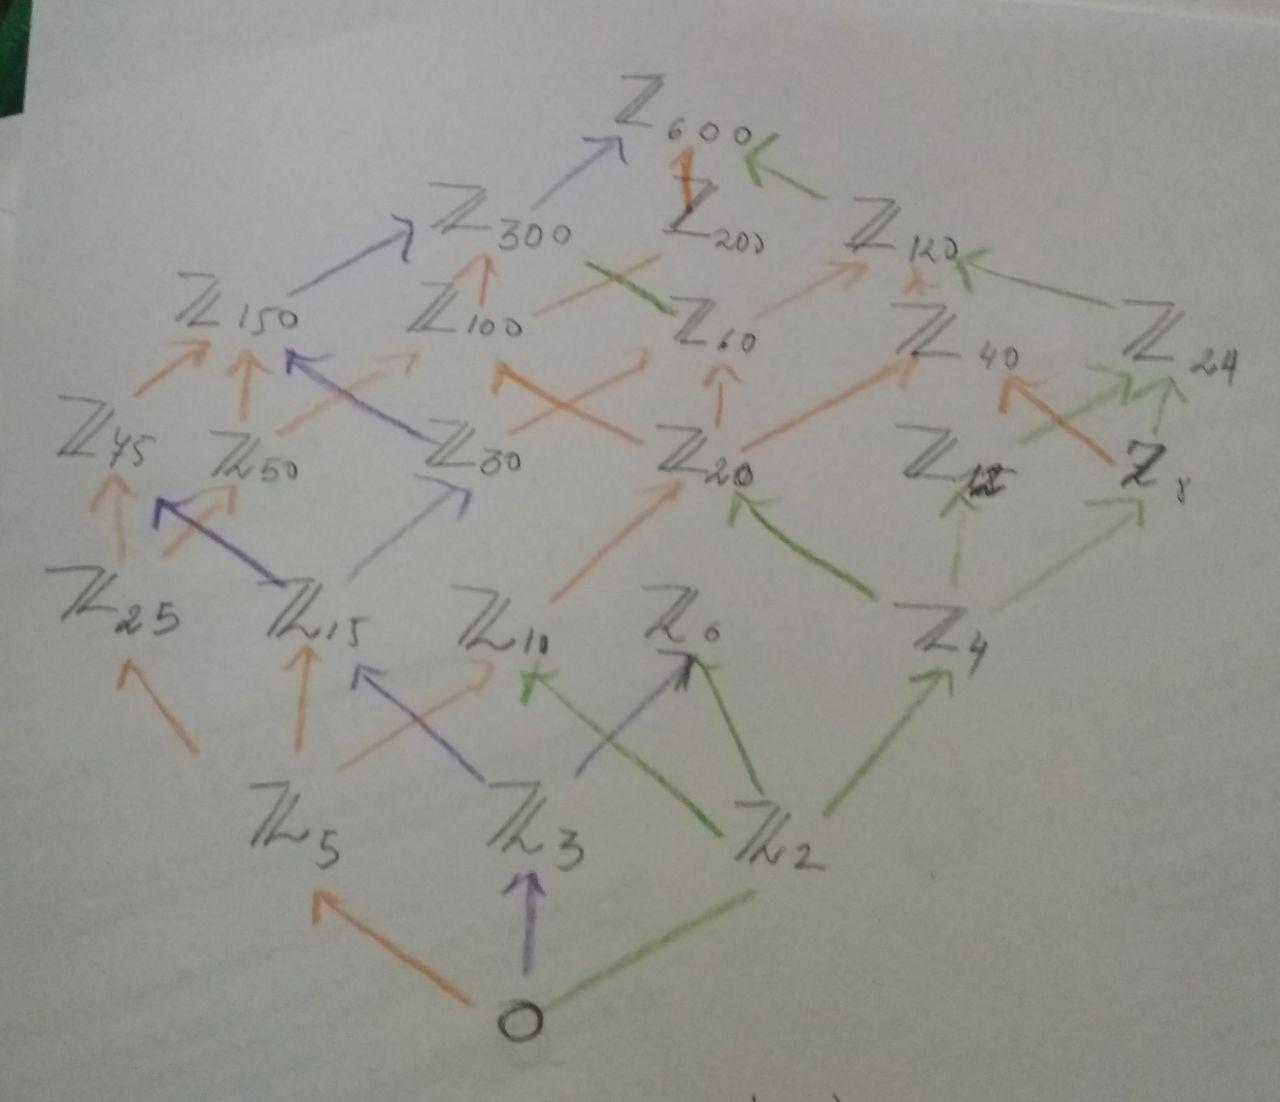
\includegraphics[width=\textwidth]{Z600}
Nota: el $0$ del grafo representa a $\{0\}$
\subsection{Apartado tercero}

\begin{micaja}
    Consideramos las permutaciones de $S_9,$
    $\sigma = (2 6)(132859)(263)$ y $\tau = (6734)(46)(37).$
    Demostrad que el subgrupo generado por ellas $<\sigma, \tau>,$ es cíclico. 
    Determine su orden y uno de sus generadores. 
\end{micaja}

Lo primero que vamos a hacer es expresar $\sigma$ y $\tau$ como ciclos disjuntos: 
\begin{itemize}
    \item $\sigma = (13859),$ que es un ciclo de longitud (y por tanto orden) 5.
    \item $\tau = (4 7),$ que es un ciclo de longitud (y por tanto orden) 2.
\end{itemize}

Si $\beta$ es una permutación
de longitud $n$ entonces $\beta^n = 1.$

Además, supongamos ahora  $\alpha$  es una permutación o composición de
permutacionens que se puede descomponer como $\alpha = a_0 a_1 ..a_r$ con $a_i$ ciclos 
disjuntos de longitud $l_i$, entonces se tiene que el $mcm(l_1,l_2..l_r)$ será el orden de la permutación,
ya que si $m = mcm(l_0, l_1,..,l_3)$  y además por ser $a_0, a_1,..,a_r$ disjuntos serán conmutativos
  se tendrá que 
$$\alpha ^m = (a_0 a_1 ..a_r)^m = a_0^m a_1^m..a_r^m = 1$$

Ya que $m$ es múltiplo de todos las longitudes y además será el orden por ser el mínimo 
número en cumplir eso. 

Y si además $l_0,l_1,...l_r$ son primos relativos, se tiene la siguiente
igualdad: 

$m_0 = mcm(l_1,..,l_r)$ (nótese que hemos quitado el primero, ni que tampoco hemos perdido
genarilidad, ya que son comnutativos podemos reordenar.)

Por tanto 
\begin{equation}
    \alpha^{m_0} = (a_0 a_1 ..a_r)^{m_0} = a_0^{m_0} a_1^{m_0}..a_r^{m_0} = a_0^{m_0}
\end{equation}



Puesto que $m_0$ será múltiplo de todos los $l_i$ salvo de $l_0.$ \paragraph{}


Y esto va a describir a las permutaciones que generen $<\alpha>$, 
ya que serán todas aquellas de la forma $s = a_0^{-L_0} a_1^{-L_1} a_r^{-L_r}$
con $L_i$ múltiplo de los $l_j$ salvo del i-ésimo y primo relativo con el resto de $L_j.$
Veamos que $<s> = <\alpha>.$

Si $\lambda = \prod_{i=0}^r Li$ se tentrá por (1) que para cualquier ciclo disjunto $a_i$

$$ a_i = s^{\frac{\lambda}{L_i}}$$
Con esto hemos probado que $<\alpha> \subseteq <s>.$ Para la otra inclusión, si 
$L_i= \prod_{i=0}^{i-1} l_i \prod_{i+1}^r l_i$ (que recordamos que eran primos relativos)
entonces el 
$$ord(<s>)= mcm(L_0,..., L_r) = L_i l_i = mcm(l_0, l_1,..., l_r) = ord(<\alpha>)$$
para cualquier $i$ subíndice de los coeficientes. 

Por lo que concluimos que $$<\alpha> = <s>$$ y es un grupo cíclico. 

\subsubsection*{Nuestro caso particular}
Vamos a elegir los $L_i$ más simples, para $\sigma$ la longitud de $\tau$ y para 
$\tau$ la de $\sigma.$ 
Por tanto 
 $$\gamma = \sigma ^{-2} \tau ^{-5} = \sigma^{5-2}\tau  = (1 5 3 9 8)(4 7)$$ 
 Se tendrá que 
 $$<\gamma> = < \sigma, \tau>$$ Por tanto $< \sigma, \tau>$ \textbf{ será un grupo cíclico 
 y uno de sus generadores será} $\gamma.$
 
 Su \textbf{orden} será el mínimo común múltiplo de las longitudes de $\sigma$ y $tau$: 

 $$ord(< \sigma, \tau>) = mcm(ord(\sigma), ord(\tau)) = mcm (5,2) = 10.$$

\subsection{Apartado cuarto}

\begin{micaja}
    Sea $n \geq 2$ y $p \leq n$ un número primo. Demostrad que en $S_n$ los únicos elementos
    de orden $p$ son los productos de ciclos disjuntos de longitud $p.$ ¿Cuántos elementos de orden
    2 tiene $S_5$?
\end{micaja}


\textbf{Condición suficiente.}\paragraph{}
 Sea $s \in S_n$  una permutación de orden $p$, si $s$ es un ciclo entonces es eviendente. 
 Si no, admitirá ser expresado como la composición de ciclos disjuntos $s = a_0..a_r$ que 
 tendrá respectivamente $l_0, ..., l_r$ órdenes, y por tanto $ord(a) = mcm(l_0,...,l_r)$
 pero claro el $ord(a) = p$ que es primo, entonces necesariamente $p = l_0 = ... = l_r.$ 

\paragraph{}
\textbf{Condición necesaria.}\paragraph{}
Por las consiceraciones sobre orden del apartado anterior, sabemos que para $s \in S_n$, 
descomponible en ciclos disjuntos de longitud $p;$ entonces su orden 
va a ser el mínimo común múltiplo del orden de sus ciclos disjuntos, pero como este es
siempre $p$ entonces el orden de $s$ es $p.$

\subsubsection*{Elementos de orden 2 en $S_5$}

En $S_5$ existe $\frac{1}{2}\frac{5!}{3!} = \frac{1}{2}5\times 4 = 10$  ciclos de orden 2 diferentes.
(hemos dividido entre dos ya que los simétricos representan la misma transposición). 

Y por el apartado anterior todos los elementos de orden 2 que existe serán producto de estos ciclo disjuntos, 
(sin que importe el orden a la hora de componer): 
Es más, no podrá contener una composición mayor de dos trasposiciones disjuntas, 
ya que si hubiera más habría algún elemento que se repetiría formando algún
ciclo mayor y ya no podría ser de orden 2 o ese caso es equivalente a uno de composición
de menos de dos juntos disjuntos (el cual ya habriamos contabilizado).

Vamos a ver cuántas permutaciones habrá como composición de dos ciclos disjuntos. 
Tomamos una de las 10 posibles $(x_0 x_1)$ y de esta nos quedarán por combinar $5-2$ elementos,
es decir $\frac{3!}{2}$ casos quitando simtrías.
Finalmente como tenemos 10 permutaciones, elimitando la mitad (por conmutatividad) $\frac{10}{2} \frac{3!}{2} = 15$ 



Con lo que concluimos que habrá elementos de orden dos: $10 + 15 = 25$ casos.

\newpage

\section{Ejercio 3}
\subsection{Apartado primero}

\begin{micaja}
    Sean las matrices de Heisenberg. 

    Demostar que $G$ es un grupo (con producto de matrices). ¿Es abeliano? ¿Es cíclico?
    ¿Es $H$ un subgrupo de $G$? En caso afirmativo, ¿Es normal en $G$?

    Probar que $f: \leftarrow \mathbb R$ defini como $f(A)=a+c$ es un homomorfismo de grupos 
\end{micaja}

\subsubsection*{G es un grupo.}

Por la caracterización de grupo debe cumplir: 

\begin{enumerate}
    \item \textbf{Existencia de un elemento neutro}, la matriz identidad pertenece a $G$ 
    (que por tanto es no vacío) y a demás es el elemento neutro. 
    \item \textbf{Propiedad asociativa.} El producto de matrices es asociativo, así que aquí 
    también lo será. 
    \item \textbf{Existencia de un elemento inverso} en $G$ para todo elemento de $G$. 
    Esto se ve fácilmente de la siquiente manera: 

    \begin{equation*}
        Sea A \in G \text{ y por tanto es de la forma } A = 
        \left(
        \begin{matrix}
            1 & a & b \\
            0 & 1 & c \\
            0 & 0 & 1
        \end{matrix}
        \right)
    \end{equation*}
    Con $a,b,c\in \mathbb{R}$

    Y queremos encontrar una matriz de la forma 
    \begin{equation*}
        B= \left(
        \begin{matrix}
            1 & x & y \\
            0 & 1 & z \\
            0 & 0 & 1
        \end{matrix}
        \right)
    \end{equation*}

    Con $x,y,z \in \mathbb{R}$ (incógnitas) que cumplan que $AB = 1$

    Por tanto lo único que nos faltaría ver es que el sistem que forman $x,y,z$ tiene solución, 
    
    las ecuaciona a las que da lugar son 

  \begin{equation*}
    \left\{
      \begin{array}{l}
         x + a = 0 \\
         y + az + b = 0 \\
         z +c = 0
      \end{array}
      \right.
  \end{equation*}


Que tienen como sulución $x = -a, z = -c, y = ac-b$
que cumplen $x,y,z \in \mathbb{R}$ y como queriamos demostrar, 
para toda matriz de $G$ existe su inversa en $G.$

\end{enumerate}

\subsubsection*{No es abeliano}


\begin{equation*}
    A B = 
    \begin{pmatrix}
        1 & a & b \\
        0 & 1 & c \\
        0 & 0 & 1
    \end{pmatrix}
    \times
    \begin{pmatrix}
        1 & x & y \\
        0 & 1 & z \\
        0 & 0 & 1
    \end{pmatrix}
    = 
    \begin{pmatrix}
    1 & x+a & y + az + b\\
    0 & 1 & z + c\\
    0 & 0 & 1
    \end{pmatrix}
\end{equation*}
\begin{equation*}
    BA = 
    \begin{pmatrix}
        1 & x & y \\
        0 & 1 & z \\
        0 & 0 & 1
    \end{pmatrix}
    \times
    \begin{pmatrix}
        1 & a & b \\
        0 & 1 & c \\
        0 & 0 & 1
    \end{pmatrix}
    = 
    \begin{pmatrix}
    1 & x+a & b + xc + y\\
    0 & 1 & z + c\\
    0 & 0 & 1
    \end{pmatrix}
\end{equation*}

la entrada $(3,3)$ es diferente, luego no es cíclico.


\subsubsection*{No es cíclico}


Vamos a verlo por la numerabilidad de $\mathbb R$
(sí, confieso que he matado moscas a cañonazos).
Que fuera cíclico supondría que $\mathbb R$ es numerable, 
ya que si existera una matriz $E \in G$, 
de tal forma que $<E>=G$, necesariamente $E$ distinta de la identidad
entonces alguna de sus entradas correspondientes a $a,b,c$ serán no nulas 
, llamemos a la posición en la matriz de esta entrada $e$.
Pues bien si ahora, considera cualquier $r \in \mathbb R$, cogemos una matriz $R$
igual a la identidad salvo en $e$ que en vez de $0$, tiene en esa casilla $r.$

Sabemos que por ser un ciclo existiría un $n$ natural tal que $E^n = R$
y por tanto habriamos encontado una inyección de los reales en los naturales, lo cual
es un contradición. 

\subsubsection*{H es un subgrupo de G}
Esto será si para todo $X,Y \in H$ se cumple que $X Y^{-1} \in H$
Por el primer apartado hemos visto que si 

\begin{equation*}
    X = 
    \begin{pmatrix}
        1 & 0 & x \\
        0 & 1 & 0 \\
        0 & 0 & 1
    \end{pmatrix}
    Y = 
    \begin{pmatrix}
        1 & 0 & y \\
        0 & 1 & 0 \\
        0 & 0 & 1
    \end{pmatrix}
\end{equation*}
entonces la inversa $Y$ será de la forma: 

\begin{equation*}
    Y = 
    \begin{pmatrix}
        1 & 0 & -y \\
        0 & 1 & 0 \\
        0 & 0 & 1
    \end{pmatrix}
\end{equation*}

y finalente

\begin{equation*}
    XY^{-1} = 
    \begin{pmatrix}
        1 & 0 & x-y \\
        0 & 1 & 0 \\
        0 & 0 & 1
    \end{pmatrix}
\end{equation*}
Que es de las formas de las matrices de $H$, por lo que es un subgrupo.

\subsubsection*{Normalidad de H en G}

$H$ será normal en $G$ si y solo si $AHA^{-1} \leq H$ para cualquier $A \in G.$
Sean cualesquieras
\begin{equation*}
    A = 
    \begin{pmatrix}
        1 & a & b \\
        0 & 1 & c \\
        0 & 0 & 1
    \end{pmatrix}
    , Y \in H, 
    Y = 
    \begin{pmatrix}
        1 & 0 & y \\
        0 & 1 & 0 \\
        0 & 0 & 1
    \end{pmatrix}
\end{equation*}

Se tiene que 
\begin{equation*}
    A H A^{-1}= 
    \begin{pmatrix}
        1 & 0 & d \\
        0 & 1 & 0\\
        0 & 0 & 1
    \end{pmatrix}
\end{equation*}

Luego $H$ es normal en $G$.
\subsubsection*{f es un homomorfismo de grupos}

Para que sea homomorfismo debe cumplir que $f(AB) = f(A)f(B)$ 
    para cualesquiera matrices $A,B \in G.$

    \begin{equation*}
        f(A)+ f(B)= 
        f 
    %    \left\( 
        \begin{pmatrix}
            1 & a &  b\\
            0 & 1 & c\\
            0 & 0 & 1
            \end{pmatrix}
           % \right\) 
           +
            f %\left\( 
        \begin{pmatrix}
            1 & x & y \\
            0 & 1 & z \\
            0 & 0 & 1
            \end{pmatrix}
            %\right\)
            = (a+c)+(x + z) 
    \end{equation*}
    y por otro lado
    \begin{equation*}
        f(AB)= 
        f %\left\( 
        \begin{pmatrix}
            1 & x+a & y + az + b\\
            0 & 1 & z + c\\
            0 & 0 & 1
            \end{pmatrix}
            %\right\) 
            = (x+a)+(z+c) 
    \end{equation*}
    
    Ambas expresiones son iguales por tanto es un homomorfismo. 

\subsubsection*{Núcleo de f}

Se define el $ker(f)$  como   $ker(f) = \left\{ e \in G | f(e) = 0\right\}$
luego 
\begin{equation*}
    ker(f) = \left\{ \begin{pmatrix}
        1 & a & b \\
        0 & 1 & -a \\
        0 & 0 & 1
        \end{pmatrix} \text{ con  } a,b \in \mathbb R\right\}
\end{equation*}

\subsubsection*{Imagen de f}

Es todo $\mathbb R$, bastará con ver que cierto conjunto de $G$
su imagen ya es $R.$

Dada una matriz de $G$ fijamos $a$ arbitrariamente
y por cómo está definida en $c$ la imagen podrá ser cualquier real. 


\subsubsection*{No es monormorfismo}
Ya que su núcleo no es la identidad.

\subsubsection*{Es epimorfismo}
Ya que $Img(f) = \mathbb R$

\newpage
\subsection{Apartado segundo}

\begin{micaja}
    Sea $f:S_4 \rightarrow S_6$ la aplicación dada por
    $f(\sigma) = \bar \sigma$, donde $\bar \sigma$
    es el elemento de $S_6$ que actúa igual que $\sigma$
    sobre los elementos $\{1,2,3,4\}$ y sobre los elementos
    $\{5,6\}$ los fija se $\sigma$ es par, o los intercambia
    si $\sigma$ es impar.

    Demostad que $f$ es un homomorfismos 
    inyectivo de grupos y que su imagen está contenida en $A_6.$
\end{micaja}

\subsubsection*{Es homomorfismo}

Para que sea homomorfismo debe cumplir que $f(ab) = f(a)f(b)$, para cualesquiera $a,b \in S_4.$

Distinguiremos los siguientes casos: 

\begin{itemize}
    \item $a,b \in S_4$ pares, entonces $ab$ es par y por tanto $f(a)f(b)=ab = f(ab).$
    \item $a,b \in S_4$ impares ambos, entonces $ab$ es par y por tanto $f(a)f(b)=a(56)b(56).$
    Como $b \in S_4$ no contendrá ni al 5 ni al 6 y será disjunto con $(56)$ por tanto podemos comutarlos
    (solo con ese, no con a.) $a(56)b(56) = ab(56)(56) = ab = f(ab)$ por ser $ab$ par.
    \item $a,b \in S_4$ con $a$ impar y $b$ par: $f(a)f(b) = a(56)b$ y aplicando de nuevo que $(56),b$ son
    disjuntos podemos conmutarlos:$a(56)b = ab(56) = f(ab)$ por ser $ab$ impar.
    \item $a,b \in S_4$ con $b$ impar y $a$ par:$f(a)f(b)= ab(56) = f(ab)$ ya que $ab$ es impar. 
\end{itemize}

\subsubsection*{Inyectividad de f}

Sean $a,b \in S_4$ tales que $f(a) = f(b).$ 
vamos a ver que necesariamente $a=b.$

\begin{equation*}
    id = f(a)f^{-1}(b) = f(a)f(b^-1) = f(ab^{-1})
\end{equation*}
Donde hemos utilizado que $f$ es un homomorfismo y ahora por cómo se ha construido $f$, 
llegamos a la igualdad $id = ab^{-1}$ de la que concluimos que $a = b$ como queriamos probar. 

\subsubsection*{Imgen de $f$ contenida en $A_6$}
El grupo alterado $An$ se define como las permutaciones pares de $Sn,$ veamos pues que 
la imagen de $f$ está formada por permutaciones pares. 


Para ello distinguiremos dos casos, ya que toda permutación es par o impar.
\begin{itemize}
    \item $a \in S_4$ par, luego $f(a) = a$ que será par. 
    \item $a \in S_4$ impar, luego $f(a) = a(56)$ que es composición de dos impares, luego será par.
\end{itemize}

\subsection{Apartado tercero}

\begin{micaja}
    
    Sea $K$ un cuerpo de $SL(K) = \{ A \in GL_n(K)/ det(A)=1\}, n \geq 2.$

    Demostrad que $SL_n(K)$ es un subgrupo normal de $GL_n(K).$ ¿Quién es el grupo cociente
    $GL_n/SL_n(K)$?

    Si $K$ es un cuerpo finito con $q$ elementos, determinad los órdenes de estos dos grupos, 
    esto es, $|GL_n(K)|$ y $|SL_n(K)|.$
\end{micaja}

\subsubsection*{$SL_n(K)$ es un subgrupo de $GL_n(K)$}

Sean cuales quiera $A,B \in SL_n(K)$, decir que el determinantes de ambos es 1. 
Por las propiedades de los determinantes: 
$det(A B{-1}) = det(A) frac{1}{det(B)} = 1$ luego  $AB^{-1} \in SL_n(K)$
y por tanto es un subgrupo. 

\subsubsection*{Normalidad}
Habremos probado que $SL_n(K)$ es un subgrupo normal de $GL_n(K)$ si para toda
$m \in GL_n(K)$, se tiene que $m SL_n(K) m^{-1} \leq SL_n(K),$ o lo que es lo mismo 
que $\{m s m^{-1} | s \in SL_n(K) \} \leq SL_n(K).$

Y esto es cierto por las propiedades de los determinantes y por
 estar $s$ en $SL_n(K)$ (ya que $det(s)=1$  ). Veámoslo: 

$det(m s m^{-1}) = det(m) det(s) \frac{1}{det(m)} = det(s) = 1.$

por tanto $msm{-1} \in SL_n(K).$

y es un subgrupo normal. 

Otra forma de verlo, más rápida que la anterior es darse cuenta 
que la definición dada de $SL(K)$ se corresponde 
con la del núcleo del determinante y esto es siempre un subgrupo normal. 

\subsubsection*{Caracterización del grupo cociente}
Vista la observación anterior y gracias al primer teorema de isomorfía tenemos que

\begin{equation}
    \frac{GL_n(K)}{SL_(K)} \cong det_*(GL_n(K)) = K^\times
\end{equation}

Nótose que no es isomofro a $K$ ya que $GL_n(K)$ son las matrices invertibles
con entradas en $K$,
es decir su determinante no puede ser nulo. 

\subsubsection*{Órdenes para $K$ finito de $q$ elementos.}

Por la caracterización del grupo cociente (2) y por ser 
$K$ un cuerpo fininto de $q$ elementos tenemos que: 

\begin{equation}
    |GL_n(K)| = (q-1) |SL_n(K)|
\end{equation}

Si hay $q$ elementos y las matrices son de $n \times n.$
Se tendrá que cada fila admite $q^n$ combinaciones, pero tenemos que tener en cuenta:
\begin{itemize}
    \item Que la primera no puede ser nula, lo cual nos deja $q^n -1$ posibilidades.
    \item Que la fila $m+1 \leq n$ no puede ser combinación lineal de las $m$ anteriores, 
    es decir que admite $q^{n}-q^{m}$
\end{itemize}

De lo que se deduce que: 
\begin{equation*}
    |GL_n(K)| = \prod_{i=0}^{n-1} (q^n - q^i)
\end{equation*}

y por (3) que si $q>1$:
\begin{equation*}
    |SL_n(K)| = \frac{1}{q-1}\prod_{i=0}^{n-1} (q^n - q^i)
\end{equation*}

El caso $q = 1$ no se puede dar ya que $n \geq 2$ y toda matriz con todas sus entradas iguales
tienen determinante 0 y no son invertibles, es decir $GL_n(k) = \emptyset.$

Esto nos sugiere además que para que la ecuaciones sean válidas, $q \leq 2$, ya que la matriz
identidad de $GL_n(k)$ tienen dos elementos y es siempre invertible. 



\newpage

\section{Ejercicio 4}

\subsection{Apartado primero}

\begin{micaja}
    Sean $A,B,C$ subgrupos de un grupo $G$ con $B \trianglelefteq A.$

    Demostrad que $B \cap C \trianglelefteq A  \cap C$ y que 

    \begin{equation*}
        \frac{A \cap C}{B \cap C} \cong \frac{B(A \cap C)}{B}
    \end{equation*}
   
\end{micaja}


\subsubsection*{$B \cap C$ es subgrupo de  $A  \cap C$ }

Por la caracterización de subgrupo
tenemo que comprobar que para cualquier $a,b \in B \cap C$ se cumple que 
$ab^{-1} \in B \cap C.$

Sean $a,b \in B \cap C$ o equivalentemente dos elemento que cumplen que
 $a,b \in B$ y $  a,b \in C$ donde $B,C$ son ambos sumbgrupos, 
 y por tanto deducimos que $ab^{-1} \in B$ y $ab^{-1} \in C$, es 
 decir que $ab^{-1} \in B \cap C$

Por hipótesis sabemos además que $B \trianglelefteq A$ luego si 
$ab^{-1} \in B$ también se tendrá que $ab^{-1} \in A;$ y como ya habíamos visto 
antes
que $ab^{-1} \in C$ entonces $ab^{-1} \in A  \cap C;$ probando con ello lo que 
buscábamos, que $B \cap C$ es subgrupo de  $A  \cap C.$


\subsection*{$B \cap C$ es subgrupo normal de  $A  \cap C$}

    Como hipótesis partimos de que $B \trianglelefteq A$ y que $A,B,C \in sub(G).$

Entonces en particular tenemos que $A \cap C$ es un subgrupo de $A$ y que $A \cap B = B.$

Con esto y una sonrisa podemos, ya que se cumplen las hipótesis del tercer teorema de isomorfía
( $B, A \cap C \leq A$ y $B \trianglelefteq A$ )
podemos afirmar que $B \cap (A \cap C) \trianglelefteq (A \cap C)$
pero claro, $B \cap (A \cap C) = (B \cap C).$

Por tanto hemos probado que 

\begin{equation*}
    B \cap C \trianglelefteq A \cap C.
\end{equation*}


Lo recién demostrado da derecho a la vida de  $\frac{A \cap C}{B \cap C}$
y por tanto a la pregunta siguiente del examen tiene sentido 
(cosa que no había dudado en ningún momento). 



\begin{micaja}
    Demuestre que 
\begin{equation*} 
    \frac{A \cap C}{B \cap C} \cong \frac{B(A \cap C)}{B}
\end{equation*}
\end{micaja}

%Antes de nada tengamos presenta la siguiente igualdad elemental de conjuntos.
%Sean $A,B$ dos conjuntos no vacío que cumplen que $B \subseteq A$ entonces $B = A \cap B.$

Hemos visto en el apartado anterior que se cuplen las hipótesis 
 del tercer teorema de isomorfía y utilizando toda la artillería llegamos 
 a las siguientes igualdades: 

 \begin{equation*}
    \frac{A \cap C}{B \cap C} = \frac{A \cap C}{B \cap (A \cap C)} \cong \frac{(A \cap C)B}{B}
    = \frac{B(A \cap C)}{B}
 \end{equation*}
\begin{itemize}
    \item Para la primera igual hemos usado la observación conjuntística.
    \item Para el primer isomorfismo, la tercera consecuencia del 
    tercer teorema de isomorfía. 
    \item Para la segunda igualdad,aprovechamos que $B \trianglelefteq A$ es decir que  $aB = Ba$ para todo $a \in A$
    entonces en particular lo será para cualquiera $a \in A\cap C$
    lo que a nivel de conjuntos se traduce en que $B(A\cap C) = (C \cap A) B.$
   
\end{itemize}
 


\begin{micaja}
    Si además $C \trianglelefteq G,$ demostrad que $BC \trianglelefteq AC$ y 

    \begin{equation*}
        \frac{AC}{AC} \cong \frac{A}{A \cap (BC).}
    \end{equation*}
\end{micaja}
    
\subsubsection*{$C \trianglelefteq G,$ demostrad que $BC \trianglelefteq AC$.}
En esta demostración utilizaré la siguiente relación de normalidad: 

Si $N \trianglelefteq S$ entonces sean cuales sean $s \in S, n \in N$ existirán $n',n'' \in N$
tales que $sn = sn'$ y $ns = sn''.$ (De hecho $n'' = n$).

Queremos probar que $BC \trianglelefteq AC$, 
esto será si para todo $ac  \in AC$ se cumple que $ac BC (ac)^{-1} \leq BC$ o 
equivalentemente que para todo $\beta \gamma \in BC$ se cumple que $ac \beta \gamma (ac)^{-1} \in BC.$

Vamos a ir operando con $ac \beta \gamma (ac)^{-1}$.
\begin{itemize}
    \item $ac \beta \gamma (ac)^{-1} = ac \beta \gamma c^{-1} a^{-1}.$
    \item $C$ es un subgrupo, y $\gamma , c \in C,$ luego existe $c_1 \in C$ tal que $c_1 = \gamma c^{-1}.$
    \item Por la observación del principio y por ser $C \trianglelefteq G$ existirá un $c_2$ tal que $c_1 a^{-1} = a^{-1}c_2.$
    Luego $ac \beta c_1 a^{-1} = ac \beta a^{-1} c_2.$
    \item Como $B \trianglelefteq A$ repetimos varias veces el razonamiento anterior. 
\end{itemize}

Finalmente llegamos a que $ac \beta \gamma (ac)^{-1} = a a^{-1} b_2 c_3$ con $b_2 \in B$, $c_3  \in C$, 
y por ende que $ac \beta \gamma (ac)^{-1} \in BC$ como queríamos ver. 

Algo notable de esta demostración es que podríamos debilitar las hipótesis iniciales, es decir
que en vez de que $C \trianglelefteq G$ nos bastaría con que $C \trianglelefteq A.$ De todas formas
utilizaremos la normalidad más estricta para el siguiente apartado. 

\begin{micaja}
    Si además $C \trianglelefteq G,$ demostrad que  

    \begin{equation*}
        \frac{AC}{AC} \cong \frac{A}{A \cap (BC).}
    \end{equation*}
\end{micaja}
    
En el contexto en que que estamos trabajando son válidas las siguientes afirmaciones: 

\begin{enumerate}
    \item Como $B \trianglelefteq A$ entonces $A = AB.$
    \item Por el apartado anterior $BC \trianglelefteq AC$ y además que $A, BC \leq AC.$
    $A \leq AC$ ya que $C$ es subgrupo y contiene al cero y por tanto para todo $a \in A$ se tiene que
     $a1 \in AC$ lo que hace que $A subset AC$
\end{enumerate}

Primero por la observación (1) y luego por la segunda obtenemos lo que queriamos demostrar.

\begin{equation*}
    \frac{AC}{BC} = \frac{ABC}{BC} = \frac{A}{A\cap (BC).}
\end{equation*}


\subsection{Apartado segundo}

\begin{micaja}
    Sea $G$ un grupo. Un subgrupo $H \leq G$ se dice que un subgrupo de Hall de $G$ si su 
    índice  en $G$ es primo relativo con su orden.

    Sea $N \triangleright G$ un subgrupo de orden de G. Demostrad que si H es un subgrupo de Hall de 
    $G$, entonces $H \cap N$ es un subgrupo de Hall de $N$ y $HN/N$ es un subgrupo de Hall de $G/N.$
\end{micaja}


\subsubsection*{$H \cap N$ es un subgrupo de Hall de $N$ }

Gracias al teorema de lagrange sabemso que $|G| = [G:H] |H| = pq$ con $p,q$ primos relativos
Se tiene que $N$ es subgrupo normal de $G$, sabemos que $1 \leq |N| \leq |G|\}.$
Por otro lado la interseción de subgrupos es un subgrupo así que $1 \in |H \cap N|$ y si 
teníamos que $|H|=p$  entonces $1 \leq |N \cap H| \leq p.$
Además el teorema de Larange nos da las siguientes igualdades:


\begin{equation}
    \left\{
      \begin{array}{l}
        |G| = [G:H] |H|\\
        |G| = [G:N] |N| \\
        |N| = [N: N \cap H] |N\cap H|   
      \end{array}
      \right.
  \end{equation}



Y queremos ver que $mcd([N: N \cap H] ,|N\cap H|) = 1.$

Como $N$ es normal se cumplen las hipótesis del teorema de Lagrange
y tenemos también que $N \cap H \trianglelefteq H$
lo que da derecho a la vida a 
$$\frac{H}{N \cap H}$$ y nos indica además que $|N\cap H|$ es 
divisor de $|H|.$

Y concatenando las igualdades de (4) tenemos la siguiente igualdad

\begin{equation*}
    [G:N] [N: N \cap H] |N\cap H|  = [G:H] |H|
\end{equation*}

Y saca a relucir que si queremos que $mcd([N: N \cap H] ,|N\cap H|) = 1$,
$[N: N \cap H]$ debe de ser únicamente producto de factores de $[G:H],$ es decir un divisor suyo.

Lo cual se cumple por la siguiente igualdad:

\begin{equation}
    [N: N \cap H] = \frac{|N|}{|N\cap H|} = \frac{|N|}{|H|}\frac{|H|}{|N\cap H|}  
    =  \frac{|N|}{|H|}\frac{|HN|}{|N|} 
\end{equation}
\begin{equation*}
    = |HN| \frac{|G:H|}{|G|} = \frac{|G:H|}{|G:HN|} 
\end{equation*}

Que ha sido deducida siguiendo estos pasos:
\begin{enumerate}
    \item Despejando el índice de la tercera ecuación de (4).
    \item Aplicando el teorema de isomorfía.
    \item Despejando $|H|$ de la primera ecuación de (4) y 
sustituyendo su valor.
    \item $NH$ es subgrupo de $G$ y por Teorema Lagrange.
\end{enumerate}

\textbf{Recapitulando}

Tenemos que  $[N: N \cap H]$ es divisor de $|G:H|$ y que
$|N\cap H|$ lo es de $H$, por tanto 

$$mcd([N: N \cap H] ,|N\cap H|) = 1$$

y hemos probado que $|N\cap H|$ es subgrupo de Hall de $H.$

\subsubsection*{$HN/N$ es un subgrupo de Hall de $G/N$}

Procederemos igual que el apartado anterior buscando factorizar en términos conocidos
$|HN/N|$ y $[HN/N : G/N].$

Por el tercer teorema de isomorfía
$$|HN/N| = \frac{|H|}{|H \cap N|}$$ luego es divisor de $H.$


Para $[HN/N : G/N]$ vamos a tener que trabajar un poquillo más: 

Sabemos por el tercer teorema de isomorfía que  $N \trianglelefteq NH$ y $N$ es normal en $G,$
por tanto $\frac{HN}{N} \leq \frac{G}{N}$ y se cumplen 
las hipótesis del segundo teorema de isomorfía, el cual
podemos aplicar tras despejar nuestro índice, del Teorema de Lagrange 

\begin{equation*}
    [HN/N : G/N] = \frac{|G/N|}{|HN/G|} = |G|/|HN|
\end{equation*}

y de la ecuación (5) del apartado anterior podemos despejar $HN$ como $|HN|= \frac{[N:N \cap H] |G|}{[G:H]}$ 
 llegando a queda

\begin{equation*}
    |G|/|HN| = |G| \frac{[G:H]}{[N:N \cap H] |G|}
\end{equation*}
Luego 

\begin{equation*}
    [HN/N : G/N] = \frac{[G:H]}{[N:N \cap H]}
\end{equation*}

y por tanto es divisor de $[G:H].$

En conclusión tenemos que: 

\begin{itemize}
    \item $|HN/N|$ divisor de $H.$
    \item $[HN/N : G/N]$ es divisor de $[G:H].$
    \item $H$ y $[G:H]$ son primos relativos. 
\end{itemize}

Luego $|HN/N|$ y $[HN/N : G/N]$ son primos relativos y 
$HN/N$ es un subgrupo de hall de $G/N.$


\subsection*{Comentario final}
Pensando el ejercicio se me ocurrió y que con una condición más fuerte, que 
me parece , que en vez de primos relaticos sean primos (a esto llamaré condición de Hall fortidicada :)  
Se tendría que gracias al teorema de lagrange  
$|G| = [G:H] |H| = pq$ con $p,q$ primos, pero es que esta informacíon va más allá,
porque cualquier otro subgrupo propio $S$ de $G$ también será un subgrupo de Hall fortificado, ya que el teorema
de Lagrange fuerza a que $|G| = [G:S] |S|$ y los únicos divisores de $|G|$ son $1,p,q,|G|$ y 
$1$ y $|G|$ no son porque el subgrupo es propio. 
\end{document}



